%\begin{figure}[h!]
%    \centering
%    \includegraphics[width=14cm, height= 7.5cm]{.png}
%    \caption{}
%    \label{fig:}
%\end{figure}

%-------------------------------------------------------------------------%
\section{Performance of the classifiers}
%-------------------------------------------------------------------------%
%\subsection{Benchmark 1: \texorpdfstring{$\Tilde{t} = 1.2$}{ } TeV and \texorpdfstring{$\Tilde{\chi}_1^0 = 600$}{ } GeV}
An initial measure to visually understand how our classifiers have performed, a simple Receiver operating characteristic (ROC) curve can be constructed. A ROC curve shows the distribution of the predicted values given between 0 and 1, as a function of FP rate versus TP rate. This allows us to understand how much error we are willing to accept/reject for a given model. The ROC curve produced for all four benchmark data is presented in Figure \ref{fig:ROC}. It is not surprising that the benchmark point inside the exclusiong curve performed the worst amongst the four datasets. What is surprising, however, is that the third benchmark set which has the closest mass parameters to the fourth benchmark set performed the best although by a narrow margin. This indicates that a lighter $\Tilde{\chi}_1^0$ is favorable over heavier ones, though it is not conclusive due to the high performance of the other classifiers. \\


\begin{figure}[htbp]
    \centering
    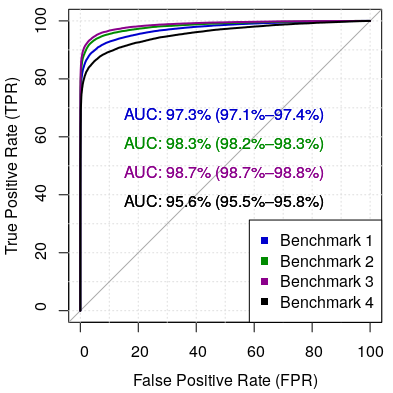
\includegraphics[width=0.4\linewidth]{ROC_curve.png}
    \caption{ROC curve for all 4 benchmark points.}
    \label{fig:ROC}
\end{figure} 

Although the Area-under-the-curve (AUC) value is given in Figure \ref{fig:ROC}, it is maximized and does not directly represent the accuracy of our models. The accuracy of our models can be obtained by setting a cut-off to our predictions i.e. a number between 0 and 1. The closer the value is to 1 the lower the accuracy, but deliberately obtaining a high accuracy by setting a smaller value is also conter-intuitive as the Signal-to-Noise Ratio (SNR) will be smaller. Through various trials in cut-off values, it was determined for all four datasets that 0.6 is the optimal value to satisfy both high accuracy and high SNR. \\

For the benchmark point $\Tilde{t} = 1.2$ TeV and $\Tilde{\chi}_1^0 = 600$ GeV, the classifier performed quite well, producing a result of above $90\%$ accuracy. It is expected that the classifier performed less accurately when dealing with signal-like events. It correctly identified a smaller portion of true signal events and incorrectly classified more signal-like background events, as seen in Table \ref{tab:Values1}. The number of expected number of signal is significantly less than the expected number of background, producing an AMS value of 0.046. Considering the definition of AMS given in Section \ref{sec:metrics}, it supports the exclusion limit in Figure \ref{fig:limits}. \\

\noindent\begin{minipage}{\textwidth}
\centering
  \begin{minipage}[htbp]{0.65\textwidth}
    \centering
    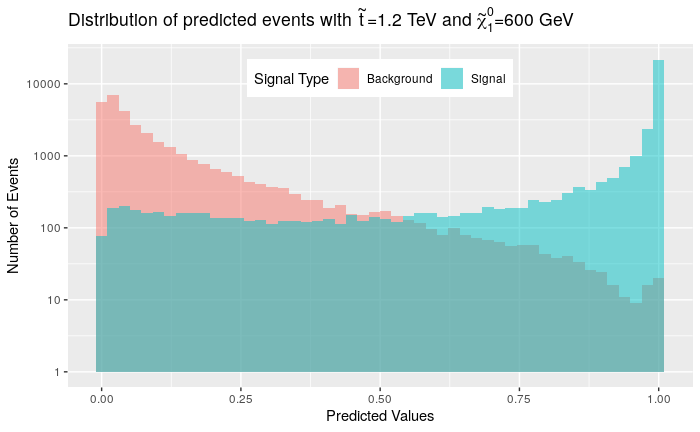
\includegraphics[width=\linewidth]{bm1_distribution.png}
    \captionof{figure}{Distribution plot for predicted values.}
    \label{fig:dist_bm1}
  \end{minipage}
  \hfill
  \begin{minipage}[htbp]{0.34\textwidth}
        \centering
        \begin{tabular}{c|c} 
        \toprule
        Metric & Proportion \\
        \midrule
        \rowcolor{gray!6} TP & $43.9 \%$ \\
        TN & $48.4 \%$ \\
        \rowcolor{gray!6} FP & $6.2 \%$\\
        FN & $1.5 \%$ \\
        \rowcolor{gray!6} Accuracy & $92.3 \pm 0.2 \%$ \\
        \midrule
        $b$ & $4328$ \\
        \rowcolor{gray!6} $s$ & $3$ \\
        SBR & $0.07\%$\\
        \rowcolor{gray!6} AMS & $0.046$ \\
        \bottomrule
        \end{tabular}
        \captionof{table}{Values for parameter $\Tilde{t} = 1.2$ TeV and $\Tilde{\chi}_1^0 = 600$ GeV.} 
        \label{tab:Values1}
    \end{minipage}
\end{minipage}
%-------------------------------------------------------------------------%
%\subsection{Benchmark 2: \texorpdfstring{$\Tilde{t} = 1.225$}{ } TeV and \texorpdfstring{$\Tilde{\chi}_1^0 = 400$}{ } GeV}

\noindent\begin{minipage}{\textwidth}
\centering
  \begin{minipage}[htbp]{0.65\textwidth}
    \centering
    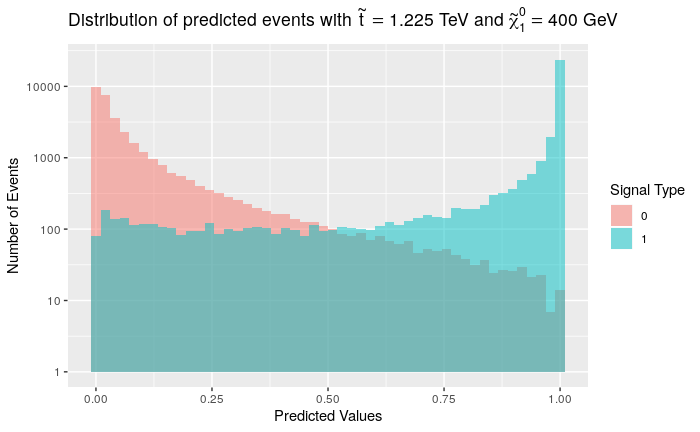
\includegraphics[width=\linewidth]{bm2_distribution.png}
    \captionof{figure}{Distribution plot for predicted values.}
    \label{fig:dist_bm2}
  \end{minipage}
  \hfill
  \begin{minipage}[htbp]{0.34\textwidth}
        \centering
        \begin{tabular}{c|c} 
        \toprule
        Metric & Proportion \\
        \midrule
        \rowcolor{gray!6} TP & $45.3 \%$ \\
        TN & $48.8 \%$ \\
        \rowcolor{gray!6} FP & $4.7 \%$\\
        FN & $1.2 \%$ \\
        \rowcolor{gray!6} Accuracy & $94.1 \pm 0.2 \%$ \\
        \midrule
        $b$ & $3250$ \\
        \rowcolor{gray!6} $s$ & $48$ \\
        SBR & $1.5\%$\\
        \rowcolor{gray!6} AMS & $0.84$ \\
        \bottomrule
        \end{tabular}
        \captionof{table}{Proportion of values of interest.} 
        \label{tab:Values2}
    \end{minipage}
\end{minipage}
%-------------------------------------------------------------------------%
%\subsection{Benchmark 3: \texorpdfstring{$\Tilde{t} = 1.25$}{ } TeV and \texorpdfstring{$\Tilde{\chi}_1^0 = 100$}{ } GeV}

\noindent\begin{minipage}{\textwidth}
\centering
  \begin{minipage}[htbp]{0.65\textwidth}
    \centering
    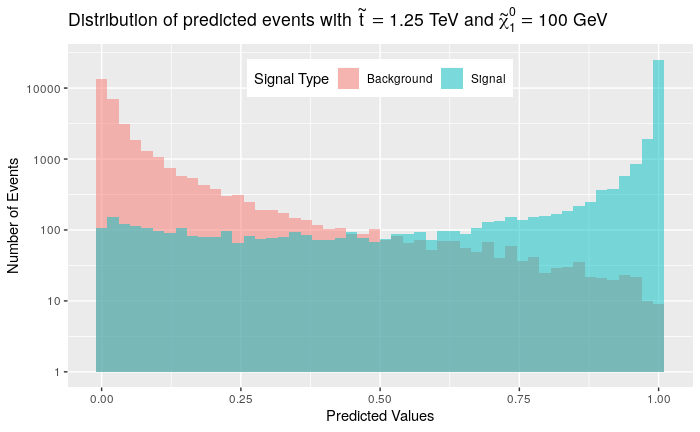
\includegraphics[width=\linewidth]{bm3_distribution.png}
    \captionof{figure}{Distribution plot for predicted values.}
    \label{fig:dist_bm3}
  \end{minipage}
  \hfill
  \begin{minipage}[htbp]{0.34\textwidth}
        \centering
        \begin{tabular}{c|c} 
        \toprule
        Metric & Proportion \\
        \midrule
        \rowcolor{gray!6} TP & $46.1 \%$ \\
        TN & $48.8 \%$ \\
        \rowcolor{gray!6} FP & $4.0 \%$\\
        FN & $1.1 \%$ \\
        \rowcolor{gray!6} Accuracy & $94.9 \pm 0.2 \%$ \\
        \midrule
        $b$ & $2798$ \\
        \rowcolor{gray!6} $s$ & $11$ \\
        SBR & $0.4\%$\\
        \rowcolor{gray!6} AMS & $0.21$ \\
        \bottomrule
        \end{tabular}
        \captionof{table}{Proportion of values of interest.} 
        \label{tab:Values3}
    \end{minipage}
\end{minipage}

%-------------------------------------------------------------------------%
%\subsection{Benchmark 4: \texorpdfstring{$\Tilde{t} = 750$}{ } GeV and \texorpdfstring{$\Tilde{\chi}_1^0 = 1$}{ } GeV}

\noindent\begin{minipage}{\textwidth}
\centering
  \begin{minipage}[htbp]{0.65\textwidth}
    \centering
    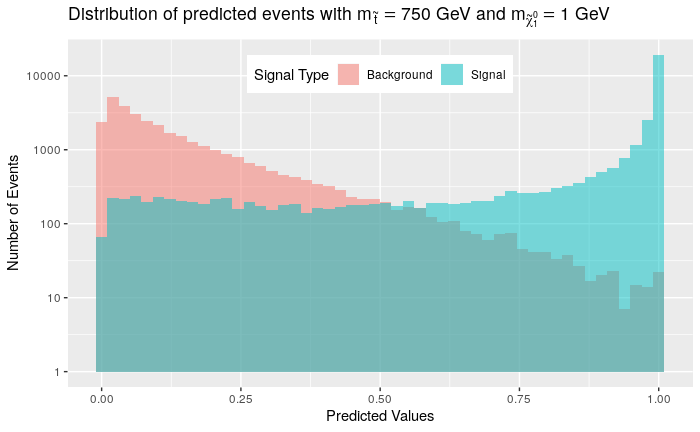
\includegraphics[width=\linewidth]{bm_In_distribution.png}
    \captionof{figure}{Distribution plot for predicted values.}
    \label{fig:dist_bm_in}
  \end{minipage}
  \hfill
  \begin{minipage}[htbp]{0.34\textwidth}
        \centering
        \begin{tabular}{c|c} 
        \toprule
        Metric & Proportion \\
        \midrule
        \rowcolor{gray!6} TP & $41.7 \%$ \\
        TN & $48.5 \%$ \\
        \rowcolor{gray!6} FP & $8.2 \%$\\
        FN & $1.6 \%$ \\
        \rowcolor{gray!6} Accuracy & $90.2 \pm 0.2 \%$ \\
        \midrule
        $b$ & $5727$ \\
        \rowcolor{gray!6} $s$ & $57$ \\
        SBR & $1\%$\\
        \rowcolor{gray!6} AMS & $0.75$ \\
        \bottomrule
        \end{tabular}
        \captionof{table}{Proportion of values of interest.} 
        \label{tab:Values_in}
    \end{minipage}
\end{minipage}

The AMS value of 0.75 obtained by this benchmark is less than but close to the value found by Roxlo and Reece \cite{roxlo2018opening} which was 1.72. This is a reassuring result, as the exclusion limit shows that indeed this point is unlikely to be the mass parameters for both the stop and the neutralino.

The result of the values may suggest that these regions will be soon excluded by the collider experiments???
%-------------------------------------------------------------------------%
\section{Data Visualisation using \textit{tourr}}

In this section, I would like to show how data visualisation could be useful in helping understand new physics beyond the SM better. By creating a two-dimensional projection of the data entailing of higher dimensions (i.e. many variables), we can observe the distribution of data points in such a projection. The \textit{tourr} package from R \cite{tourr} is an ideal program for such a task, producing interesting results. The projected tour requires an index to minimize the distance between certain points in a dataset, in which we chose to utilize the \textit{alpha-hull} index. A corresponding basis is generated with each projection, and the algorithm will search through potentially more optimal projections through each iteration. NEED TO EXPLAIN ABOUT ALPHA INDEX A BIT AND SHOW SOME SPLOTS AND TALK ABOUT THE PHYSICS WE CAN INTERPRET FROM IT.


  \begin{table}[htbp]
        \centering
        \begin{tabular}{c||c|c|c|c}
        \toprule
        &\multicolumn{1}{c|}{\bfseries Benchmark1}  &
        \multicolumn{1}{c|}{\bfseries Benchmark2}  &
        \multicolumn{1}{c|}{\bfseries Benchmark3} &
        \multicolumn{1}{c}{\bfseries Benchmark4} \\
        \midrule
        %----------------------------------%
        \textbf{Metric} & Proportion & Proportion & Proportion & Proportion \\
        \midrule
        \rowcolor{gray!6} TP & $42.0 \%$ & $43.8 \%$ & $44.9 \%$ & $39.3 \%$ \\
        TN & $49.4 \%$ & $49.5 \%$ & $49.4 \%$ & $49.5 \%$ \\
        \rowcolor{gray!6} FP & $0.6 \%$ & $0.5 \%$ & $0.6 \%$ & $0.5 \%$\\
        FN & $8.0 \%$ & $6.2 \%$ & $5.1 \%$ & $10.7 \%$ \\
        \rowcolor{gray!6} Accuracy & $91.3 \pm 0.2 \%$ & $93.3 \pm 0.2 \%$ & $94.2 \pm 0.2 \%$ & $88.8 \pm 0.2 \%$ \\
        \midrule
        $b$ & $403$ & $368$ & $371$ & $382$ \\
        \rowcolor{gray!6} $s$ & $2$ & $46$ & $11$ & $53$ \\
        SBR & $0.5\%$ & $12.5\%$ & $3.0\%$ & $13.9\%$\\
        \rowcolor{gray!6} AMS & $0.098$ & $2.32$ & $0.56$ & $2.62$ \\
        \bottomrule
        \end{tabular}
        \caption*{Proportion of important values obtained in the four benchmark parameters.}
    \end{table}